\switchcolumn[1]*
\begin{figure}[!h]
  \centering
  \begin{minipage}[t]{0.485\linewidth}
    \centering
    \textbf{Full}
  \end{minipage}
  \hfill
  \begin{minipage}[t]{0.485\linewidth}
    \centering
    \textbf{KFAC}
  \end{minipage}
  \\
  \begin{minipage}[t]{0.485\linewidth}
    \centering
    GGN ($\cvec$)\vspace{1ex}
    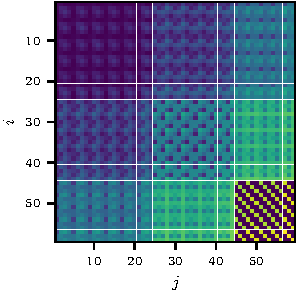
\includegraphics[width=1.0\linewidth]{../kfs/plots/synthetic_cvec_ggn_full.pdf}
  \end{minipage}
  \hfill
  \begin{minipage}[t]{0.485\linewidth}
    \centering
    GGN ($\cvec$)\vspace{1ex}
    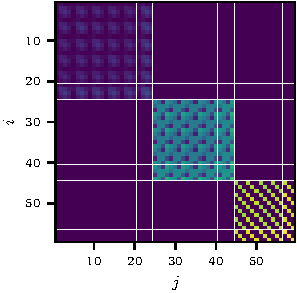
\includegraphics[width=1.0\linewidth]{../kfs/plots/synthetic_cvec_ggn_kfac.pdf}
  \end{minipage}
  \\
  \begin{minipage}[t]{0.485\linewidth}
    \centering
    MC-Fisher ($\cvec$)\vspace{1ex}
    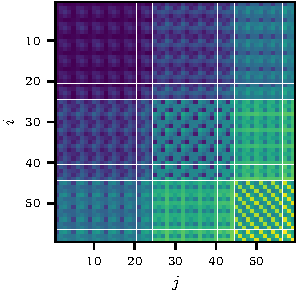
\includegraphics[width=1.0\linewidth]{../kfs/plots/synthetic_cvec_mcfisher_100_full.pdf}
  \end{minipage}
  \hfill
  \begin{minipage}[t]{0.485\linewidth}
    \centering
    MC-Fisher ($\cvec$)\vspace{1ex}
    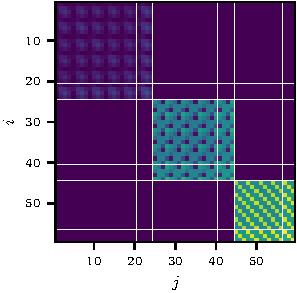
\includegraphics[width=1.0\linewidth]{../kfs/plots/synthetic_cvec_mcfisher_100_kfac.pdf}
  \end{minipage}
  \\
  \begin{minipage}[t]{0.485\linewidth}
    \centering
    Emp-Fisher ($\cvec$)\vspace{1ex}
    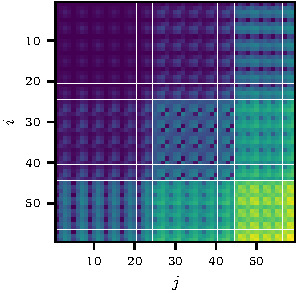
\includegraphics[width=1.0\linewidth]{../kfs/plots/synthetic_cvec_empfisher_full.pdf}
  \end{minipage}
  \hfill
  \begin{minipage}[t]{0.485\linewidth}
    \centering
    Emp-Fisher ($\cvec$)\vspace{1ex}
    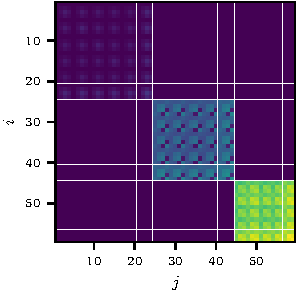
\includegraphics[width=1.0\linewidth]{../kfs/plots/synthetic_cvec_empfisher_kfac.pdf}
  \end{minipage}
  \caption{\textbf{Full curvatures and their corresponding KFAC approximation using $\cvec$-flattening}.
    All curvatures were evaluated on synthetic data ($N = 100$) using an MLP with three fully-connected layers and ReLU activations (5-4-4-3) and square loss.
    For the MC-sampled Fisher, we consider $M = 100$ samples.
    This follows the setup in \Cref{fig:hessian-block-structure}.
    KFAC concatenates the weight and bias of each layer.
    Produced with \repofile{plots/synthetic_kfac}.}
  \label{fig:cvec-kfac-full-comparison}
\end{figure}
\switchcolumn[0]

Building on the scaffold and code from the previous chapter, we now introduce, implement, and test the KFAC approximation for the weights (or combined weights and bias) of fully-connected layers (\texttt{torch.nn.Linear}).
See \Cref{fig:rvec-kfac-full-comparison,fig:cvec-kfac-full-comparison} for visualizations.

Our discussion will primarily center on regression settings with deep linear networks---MLPs composed of dense layers without nonlinearities.
This setting provides an ideal framework for understanding the core approximations behind KFAC and verifying them numerically through rigorous testing.
We focus on the formulation from \citet{martens2015optimizing}, which was originally introduced for standard MLP architectures, where linear layers do not exhibit weight sharing.

Other layers, like convolutions and linear layers inside the attention mechanism, exhibit weight sharing.
We deliberately exclude these aspects here and focus on linear layers without weight sharing.
Future versions of this tutorial may include them.

\switchcolumn[1]
\begin{figure}[!h]
  \centering
  \begin{minipage}[t]{0.485\linewidth}
    \centering
    \textbf{Full}
  \end{minipage}
  \hfill
  \begin{minipage}[t]{0.485\linewidth}
    \centering
    \textbf{KFAC}
  \end{minipage}
  \\
  \begin{minipage}[t]{0.485\linewidth}
    \centering
    GGN ($\rvec$)\vspace{1ex}
    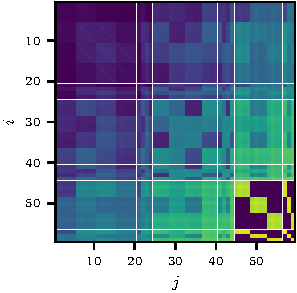
\includegraphics[width=\linewidth]{../kfs/plots/synthetic_rvec_ggn_full.pdf}
  \end{minipage}
  \hfill
  \begin{minipage}[t]{0.485\linewidth}
    \centering
    GGN ($\rvec$)\vspace{1ex}
    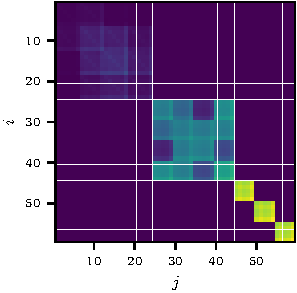
\includegraphics[width=\linewidth]{../kfs/plots/synthetic_rvec_ggn_kfac.pdf}
  \end{minipage}
  \\
  \begin{minipage}[t]{0.485\linewidth}
    \centering
    MC-Fisher ($\rvec$)\vspace{1ex}
    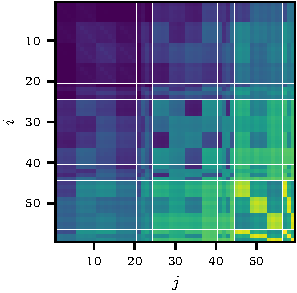
\includegraphics[width=\linewidth]{../kfs/plots/synthetic_rvec_mcfisher_100_full.pdf}
  \end{minipage}
  \hfill
  \begin{minipage}[t]{0.485\linewidth}
    \centering
    MC-Fisher ($\rvec$)\vspace{1ex}
    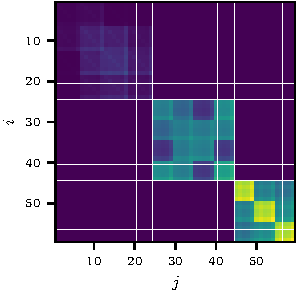
\includegraphics[width=\linewidth]{../kfs/plots/synthetic_rvec_mcfisher_100_kfac.pdf}
  \end{minipage}
  \\
  \begin{minipage}[t]{0.485\linewidth}
    \centering
    Emp-Fisher ($\rvec$)\vspace{1ex}
    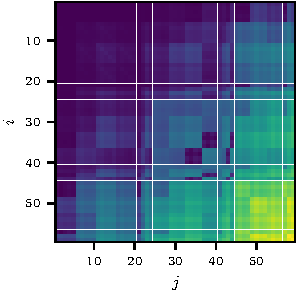
\includegraphics[width=\linewidth]{../kfs/plots/synthetic_rvec_empfisher_full.pdf}
  \end{minipage}
  \hfill
  \begin{minipage}[t]{0.485\linewidth}
    \centering
    Emp-Fisher ($\rvec$)\vspace{1ex}
    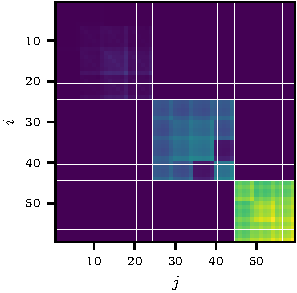
\includegraphics[width=\linewidth]{../kfs/plots/synthetic_rvec_empfisher_kfac.pdf}
  \end{minipage}
  \caption{\textbf{Full curvatures and their corresponding KFAC approximation using $\rvec$-flattening.}
    All curvatures were evaluated on synthetic data ($N = 100$) using an MLP with three fully-connected layers and ReLU activations (5-4-4-3) and square loss.
    For the MC-sampled Fisher, we consider $M = 100$ Monte Carlo samples.
    This follows the setup in \Cref{fig:hessian-block-structure}.
    KFAC concatenates the weight and bias of each layer.
    Produced with \repofile{plots/synthetic_kfac}.}
  \label{fig:rvec-kfac-full-comparison}
\end{figure}

\switchcolumn[0]

Let's formalize the layer whose curvature we approximate with KFAC in this chapter:

\begin{setup}[Linear layer inside a neural net]\label{setup:linear_layer}
  Consider a linear layer with weights $\mW \in \sR^{D_{\text{out}}\times D_{\text{in}}}$ and bias $\vb \in \sR^{D_{\text{out}}}$ in a neural net $f(\cdot, \vtheta)$.
  The network's prediction feeds into a criterion function, and we compute an empirical risk over a dataset of $N$ points, incorporating a reduction factor $R$.
  Our goal is to approximate the curvature matrix block $\mC(\vec \mW)$.

  For each datum $n$, the layer processes an input vector $\vx_n \in \sR^{D_{\text{in}}}$, producing an output vector $\vz_{n} \in \sR^{D_{\text{out}}}$ as follows
  $$ \vz_{n} = \mW \vx_{n} + \vb\,.$$
  Denote the network's prediction for datum $n$ by $\vf_n \in \sR^{\dim(\gF)}$.
  For each backprograted vector $\blacktriangle_{n,c} \in \sR^{\dim(\gF)}$, we denote the layer's output gradient as
  $$\vg_{n,c} = (\jac_{\vz_{n}} \vf_n)^{\top} \blacktriangle_{n,c} \in \sR^{D_{\text{out}}}\,.$$

  We will often neglect the bias and focus on approximating the curvature for the weight matrix $\mW$ alone.
  The bias can always be incorporated into the weight matrix by concatenation into a single weight matrix $\tilde{\mW}$ and by augmenting the input vectors with an additional constant:
  \begin{align*}
    \tilde{\mW} &= \begin{pmatrix} \mW & \vb \end{pmatrix} \in \sR^{D_{\text{out}} \times (D_{\text{in}} + 1)}\,, \\
    \tilde{\vx} &= \begin{pmatrix} \vx \\ 1 \end{pmatrix} \in \sR^{D_{\text{in}} + 1}\,.
  \end{align*}
  Thus, the derivations below hold equivalently for $\tilde{\mW}, \tilde{\vx}$ in place of $\mW, \vx$.
\end{setup}


% \begin{caveat}
%   In many modern neural networks, a linear layer processes a sequence of $S$ input vectors, transforming $(\vx_{n,1}, \dots, \vx_{n, S})$ into corresponding outputs $(\vz_{n, 1}, \dots, \vz_{n, S})$.
%   This is known as a linear layer with \emph{weight sharing}, and a key distinction arises depending on whether the layer processes each sequence element independently or not.
%   \begin{itemize}
%   \item \textbf{Independent processing:} The sequence dimension $S$ can be merged with the batch dimension $N$, effectively treating the inputs as a larger batch.
%   \item \textbf{Non-independent processing:} In cases like convolutional layers with additional pooling, the sequence elements interact, and special handling is required.
%   \end{itemize}

%   For a more detailed discussion on challenges associated with general weight-sharing, see~\citet{eschenhagen2023kroneckerfactored}.
% \end{caveat}


\subsection{Derivation of KFAC}

We now derive the KFAC approximation for a linear layer with weights $\mW$, input vector $\vx$, and output vector $\vz = \mW\vx$ (\Cref{setup:linear_layer}).
Following convention in the literature, we assume column-major ($\cvec$) flattening.

\paragraph{Exact curvature matrix.}
Recall from \Cref{eq:common-structure} that the curvature matrix \wrt $\mW$ takes the form
\begin{align*}
  &\mC(\cvec \mW) \\
  &\begin{aligned}=
    R \sum_n \sum_c &(\jac^{\cvec}_{\mW}\vz_n)^{\top} \\
                    &(\jac^{\cvec}_{\vz_n}\vf_n)^{\top}
                      \blacktriangle_{n,c} \blacktriangle_{n,c}^{\top}
                      (\jac^{\cvec}_{\vz_n}\vf_n) \\
                    &(\jac^{\cvec}_{\mW}\vz_n)\,.
  \end{aligned}
\end{align*}
We recall from \Cref{ex:linear_layer_jacobians} that the Jacobian of a linear layer's output \wrt its weights is
$$ \jac^{\cvec}_{\mW}\vz_n = \vx_n^{\top} \otimes \mI_{D_{\text{out}}}\, $$
where $\vx_n \in \R^{D_\text{in}}$ is the layer's input.
With that, and using the Kronecker product properties from \Cref{sec:mem_comp_eff_kron}, we see that the curvature matrix is a sum of Kronecker products:
\begin{align*}
  &\mC(\cvec \mW)
  \\
  &\begin{aligned}
    = R \sum_n \sum_c &(\vx_n \otimes \mI_{D_{\text{out}}}) \vg_{n,c} \\
                      & \vg_{n,c}^{\top} (\vx_n^{\top} \otimes \mI_{D_{\text{out}}})
  \end{aligned}\\
  &\begin{aligned}
    = R \sum_n \sum_c &(\vx_n \otimes \mI_{D_{\text{out}}}) \vg_{n,c} \\
                      &\left[(\vx_n \otimes \mI_{D_{\text{out}}}) \vg_{n,c} \right]^{\top}
  \end{aligned}\\
  &\begin{aligned}
    = R \sum_n \sum_c &\left( \vx_n \otimes \vg_{n,c} \right)\left( \vx_n \otimes \vg_{n,c} \right)^{\top}
  \end{aligned}\\
  &= R \sum_n \sum_c \left( \vx_n \otimes \vg_{n,c} \right)
    \left( \vx_n^{\top} \otimes \vg_{n,c}^{\top} \right) \\
  &= R \sum_n \sum_c \left(\vx_n \vx_n^{\top}\right) \otimes \left(\vg_{n,c} \vg_{n,c}^{\top}\right)\,.
\end{align*}

\switchcolumn[1]*
\begin{example}[Motivation for KFAC's expectation approximation]
  \label{ex:just_kfac_exp_approx}
  KFAC's expectation approximation can be derived from an optimality condition under specific assumptions to preserve a Kronecker structure.

  Consider the curvature matrix
  \begin{align*}
    \mC
    &=
      \textstyle
      R \sum_{n=1}^N
      (\vx_n \otimes \mI_{D_{\text{out}}})
      \vg_n \vg_n^{\top}
      (\vx_n^{\top} \otimes \mI_{D_{\text{out}}})\,.
  \end{align*}
  Our goal is to approximate $\mC$ with a single Kronecker product.

  To make this expression more compact, stack the vectors $\vx_n$ and $\vg_n$ into matrices:
  \begin{align*}
    \mX
    &=
      \begin{pmatrix}
        \vx_1 & \vx_2 & \ldots & \vx_N
      \end{pmatrix}
      \in \sR^{D_{\text{in}} \times N}\,,
    \\
    \mG
    &=
      \begin{pmatrix}
        \vg_1 & \vg_2 & \ldots & \vg_N
      \end{pmatrix}
      \in \sR^{D_{\text{out}} \times N}\,.
  \end{align*}
  and rewrite $\mC$ in terms of these matrices:
  \begin{align*}
    \mC = R (\mX \otimes \mI_{D_{\text{out}}}) \cvec(\mG) \cvec(\mG)^{\top}(\mX^{\top} \otimes \mI_{D_{\text{out}}}).
  \end{align*}
  Looking at this expression, we realize that an easy way to achieve a single Kronecker product is to approximate $\cvec(\mG) \cvec(\mG)^{\top} \approx \mI_{D_{\text{in}}} \otimes \mB$ with $\mB \in \sR^{D_{\text{out}}\times D_{\text{out}}}$.
  Then we would have
  \begin{align*}
    \mC
    &\approx
      R (\mX \otimes \mI_{D_{\text{out}}})
      (\mI_{D_{\text{in}}} \otimes \mB)
      (\mX^{\top} \otimes \mI_{D_{\text{out}}})
    \\
    &=
      R \mX \mX^{\top} \otimes \mB
      =
      \textstyle
      R \left(\sum_{n=1}^N \vx_n \vx_n^{\top}\right) \otimes \mB\,.
  \end{align*}
  To obtain $\mB$, we minimize the squared Frobenius norm residual:
  \begin{align*}
    \begin{split}
      &\argmin_{\mB}
        \left\lVert
        \cvec(\mG) \cvec(\mG)^{\top} - \mI_{D_{\text{in}}} \otimes \mB
        \right\rVert_2^2.
    \end{split}
    \intertext{Expanding the Kronecker structure, this is equivalent to}
    \begin{split}
      &\argmin_{\mB}
        \left\lVert
        \begin{pmatrix}
          \vg_1 \vg_1^{\top} -\mB & \dots & \vg_1 \vg_N^{\top} \\
          \vdots & \ddots & \vdots \\
          \vg_N \vg_1^{\top} & \dots & \vg_N \vg_N^{\top} - \mB \\
        \end{pmatrix}
        \right\rVert_2^2
      \\
      &=
        \argmin_{\mB}
        \left\lVert
        \begin{pmatrix}
          \vg_1 \vg_1^{\top} - \mB & \dots & \vzero \\
          \vdots & \ddots & \vdots \\
          \vzero & \hdots & \vg_N \vg_N^{\top} - \mB \\
        \end{pmatrix}
        \right\rVert_2^2
      \\
      &=
        \argmin_{\mB}
        \sum_{n=1}^N
        \left\lVert
        \vg_n \vg_n^{\top} - \mB
        \right\rVert_2^2
      \\
      &=
        \argmin_{\mB}
        \sum_{n=1}^N
        \sum_{i,j = 1}^{D_{\text{out}}}
        \left(
        [\vg_n]_i [\vg_n]_j - [\mB]_{i,j}
        \right)^2 \,.
    \end{split}
  \end{align*}
  Taking the derivative \wrt $\mB$ and setting it to zero yields for all $k, l \in \{1, \dots, D_{\text{out}}\}$,
  \begin{align*}
    &\frac{\partial \left(
      \sum_{n=1}^N
      \sum_{i,j = 1}^{D_{\text{out}}}
      \left(
      [\vg_n]_i [\vg_n]_j - [\mB]_{i,j}
      \right)^2
      \right)
      }{
      \partial [\mB]_{k,l}
      }
    \\
    &=
      2 \sum_{n=1}^N
      \left(
      [\mB]_{k,l} -  [\vg_n]_k [\vg_n]_l
      \right)
    \\
    &=
      2 \left( N[\mB]_{k,l} - \sum_{n=1}^N [\vg_n]_k [\vg_n]_l \right)
      \stackrel{!}{=} 0
    \\
    &\implies
      \mB = \frac{1}{N} \sum_{n=1}^N \vg_n \vg_n^{\top}
      = \frac{1}{N} \mG \mG^{\top}.
  \end{align*}
  Thus, under this optimality condition, the best choice for $\mB$ is the empirical covariance of the gradient vectors:
  \begin{align*}
    \mC
    \approx
    \left(R \sum_n \vx_n \vx_n^\top \right)
    \otimes
    \left(\frac{1}{N} \sum_{n'} \vg_{n'} \vg_{n'}^\top \right).
  \end{align*}
  This is precisely the expectation approximation used in KFAC.
\end{example}
\switchcolumn[0]

\paragraph{From sum of Kronecker products to single Kronecker product.}
The last step is to approximate the sum of Kronecker products by a single Kronecker product.
To do that, we use the so-called KFAC's expectation approximation (see \Cref{ex:just_kfac_exp_approx} for further motivation):

\begin{definition}[KFAC's expectation approximation]
  \label{def:kfac_exp_approx}
  Consider two sets of $N$ vectors $\{\vx_{n}\}_{n=1}^N$ and $\{\vg_{n}\}_{n=1}^N$ where each $\vx_n$ is input-based and each $\vg_n$ is output-gradient-based.
  KFAC approximates the sum of Kronecker products of their self-outer products by a single Kronecker product, using the following expectation approximation:
  \begin{subequations}\label{eq:expectation_approximation}
    \begin{align}
      \begin{split}
        &\sum_{n=1}^{\textcolor{VectorOrange}{N}} \vx_n\vx_n^{\top} \otimes \vg_n \vg_n^{\top}
        \\
        &\qquad\approx
          \left( \sum_{n=1}^N \vx_n \vx_n^{\top} \right)
          \otimes
          \frac{
          \left( \textcolor{VectorOrange}{\sum_n} \vg_n \vg_n^{\top} \right)
          }{\textcolor{VectorOrange}{N}}.
      \end{split}
      \intertext{In words, we sum the outer products on the left and right of the Kronecker product independently and divide by the number of outer products in the term containing the gradient vectors.
      In expectation notation (expectation meaning averaging over all values of $n$, \ie $\E_n[\bullet_n] = \nicefrac{1}{N} \sum_{n=1}^N \bullet_n$), we can write this approximation more conveniently as}
      \begin{split}
        &\E_n \left[ \vx_n \vx_n^{\top} \otimes \vg_n \vg_n^{\top} \right]
        \\
        &\qquad\approx N
          \E_n \left[ \vx_n \vx_n^{\top} \right]
          \otimes
          \E_n \left[ \vg_n \vg_n^{\top} \right]\,,
      \end{split}
    \end{align}
  \end{subequations}
  \ie `pull' the expectation into the Kronecker factors.
\end{definition}

Applying \Cref{def:kfac_exp_approx}, we obtain the curvature matrix's KFAC approximation:
\begin{align*}
  \mC&(\cvec \mW) \\
  \approx&
           \underbrace{\left( R \sum_n \vx_n \vx_n^{\top} \right)}_{\text{input-based}}
           \otimes
           \underbrace{\left( \frac{1}{N} \sum_n \sum_c \vg_{n,c} \vg_{n,c}^{\top} \right)}_{\text{grad-output-based}}
  \\
  =& \kfac(\mC(\cvec \mW))\,.
\end{align*}

\paragraph{Changing flattening swaps the Kronecker factors.}
Had we done the same derivation using the $\rvec$-flattening scheme where the output-parameter Jacobian takes the form (\Cref{ex:linear_layer_jacobians})
$$ \jac^{\rvec}_{\mW}\vz_n = \mI_{D_{\text{out}}} \otimes \vx_n^{\top}\,,$$
we would have found the order of Kronecker factors to reverse,
\begin{align*}
  \mC&(\rvec \mW) \\
  \approx&
           \left( \frac{1}{N} \sum_n \sum_c \vg_{n,c} \vg_{n,c}^{\top} \right)
           \otimes
           \left( R \sum_n \vx_n \vx_n^{\top} \right)
  \\
  =& \kfac(\mC(\rvec \mW))\,.
\end{align*}
This is important to keep in mind for KFAC implementations, as libraries like PyTorch use $\rvec$-flattening.
In summary, we have the following:

\switchcolumn[1]
\codeblock{kfac/expand_Linear}
\switchcolumn[0]

\begin{definition}[KFAC for a linear layer without weight sharing, \Cref{kfac/expand_Linear}]\label{def:kfac_expand_linear}
  Consider a linear layer inside a neural network from \Cref{setup:linear_layer}.
  The \emph{KFAC approximation} of a curvature matrix \wrt the layer's weights is given by
  \begin{subequations}\label{eq:kfac_expand_linear}
    \begin{align}
      \begin{split}
        &\kfac(\vec \mW) \approx \mC(\vec \mW)
        \\
        &\quad=
          \begin{cases}
            \mA \otimes \mB & \vec = \cvec
            \\
            \mB \otimes \mA & \vec = \rvec
          \end{cases}\,,
      \end{split}
    \end{align}
    with the input-based factor
    \begin{align}
      \mA &= R \sum_{n=1}^N \vx_{n} \vx_{n}^{\top}\in \sR^{D_{\text{in}} \times D_{\text{in}}}
                        \intertext{and the output-gradient-based factor}
                        \mB &= \frac{1}{N}\sum_{n=1}^N \sum_c \vg_{n,c} \vg_{n,c}^{\top}\in \sR^{D_{\text{out}} \times D_{\text{out}}}
    \end{align}
  \end{subequations}
  and $\vg_{n,c}$ the backpropagated vector of a curvature matrix at layer output $\vz$ given by $$\vg_{n,c} = (\jac_{\vz_{n,s}}^{\vec}\vf_n)^{\top} \blacktriangle_{n,c}\,.$$
\end{definition}

% NOTE This part is about weight sharing, which will not be in the first version.
\begin{comment}
  Similarly, we can justify flattening an additional sequence dimension into the batch dimension when no additional reduction occurs along any axes in the neural network.

  To see this, consider a sequence of input vectors represented as a matrix-valued input
  \begin{align*}
    \mX_n = (\vx_{n, 1}, \dots, \vx_{n, s}),
  \end{align*}
  where $S$ is the sequence length.
  The corresponding sequence of output vectors is given by:
  \begin{align*}
    \mZ_n = \left( \vz_{n, 1}, \dots, \vz_{n,s} \right),
  \end{align*}
  and the backpropagated vectors, regardless of their specific type, are stored in the matrix
  \begin{align*}
    \mG_{n, c} = (\vg_{n, c, 1}, \dots, \vg_{n, c, s}).
  \end{align*}
  Then, the curvature matrix takes the form:
  \begin{align*}
    \mC(&\cvec \mW) \\
        &\begin{aligned}
          =R\sum_n \sum_c \sum_s
          &(\jac^{\cvec}_{\mW}\vz_{n,s})^{\top} \\
          &\cvec\vg_{n,c,s} (\cvec\vg_{n,c,s})^{\top} \\
          &\jac^{\cvec}_{\mW}\vg_{n,c,s}
        \end{aligned}\\
        &\begin{aligned}
          = R \sum_n \sum_c &(\mX_n \otimes \mI_{\vz_n}) \\
                            &\cvec \mG_{n,c}(\cvec \mG_{n,c})^{\top} \\
                            &(\mX_n^{\top} \otimes \mI_{\vz_n}).
        \end{aligned}
  \end{align*}
  A key observation is that the matrix $\vec\mG_{n,c} (\vec\mG_{n,c})^{\top}$ has dimensions $S D_{\text{out}} \times S D_{\text{out}}$ and does not simplify into a single Kronecker product.

  Similar to Example~\ref{ex:just_kfac_exp_approx}, we would like to find an approximation
  \begin{align*}
    \cvec\mG_{n,c} (\cvec\mG_{n,c})^{\top} \approx \mK \otimes \mI_{D_\text{out}}
  \end{align*}
  to simplify the expression into a single Kronecker structure.

  Using the same optimality condition and arguments, it is straightforward to show that:
  \begin{align*}
    \argmin_{\mK}
    &\left\lVert
      \cvec \mG_{n,c} (\cvec \mG_{n,c})^{\top} - \mK \otimes \mI_{D_{\text{out}}}
      \right\rVert_2 \\
    &=
      \frac{1}{S} \mG_{n,c} \mG_{n,c}^{\top}.
  \end{align*}
  This result tells us that the optimal Kronecker approximation is again obtained by averaging the diagonal blocks of size $S\times S$, simplifying the curvature matrix to:
  \begin{align*}
    \mC(\cvec\mW)
    &\approx
      R \sum_n \sum_c
      \mZ_n \mZ_n^{\top} \otimes \frac{1}{S} \mG_{n,c} \mG_{n,c}^{\top}
    \\
    &= R \sum_n \sum_s \vz_{n,s} \vz_{n,s}^{\top} \\
    &\quad\otimes \sum_{s'} \sum_c \frac{1}{S} \vg_{n,s',c} \vg_{n,s',c}^{\top}
      \intertext{Applying KFAC's expectation approximation from \Cref{def:kfac_exp_approx}, we obtain}
    &\approx
      \left(R \sum_n \sum_s \vz_{n,s} \vz_{n,s}^{\top}\right)
    \\
    &\quad\otimes \left( \frac{\textcolor{VectorOrange}{\sum_n} \textcolor{VectorTeal}{\sum_s}\sum_c \vg_{n,s,c} \vg_{n,s,c}^{\top}}{\textcolor{VectorOrange}{N} \textcolor{VectorTeal}{S}} \right).
  \end{align*}
  This equation highlights that the sequence dimension (highlighted in \textcolor{VectorTeal}{teal}) is treated exactly like the batch dimension (highlighted in \textcolor{VectorOrange}{orange}) in KFAC's expectation approximation.
  Consequently, if no additional reduction occurs along the sequence dimension, it can be flattened into the batch dimension without affecting the approximation structure.
\end{comment}

\subsection{Tests}

To verify our KFAC implementation, we need tests.
This raises an important question: When does the approximation in \Cref{eq:expectation_approximation} become exact?
In general, KFAC's expectation approximation becomes exact whenever one of $\{\vx_n\}_n$ or $\{\vg_{n,c}\}_{n,c}$ is data-independent, \ie, does not depend on $n$.
There are two notable cases where this happens, one of which is relatively obvious.

\switchcolumn[1]
\codeblock{kfac_tests/mlp_batch_size_1}
\switchcolumn[0]

\subsubsection{Data Set Size 1}
A particularly straightforward case occurs when summation over $n$ disappears, \ie when the dataset is only a single data point or $N$ identical data points.
Hence, we have the following

\begin{test}[KFAC for linear layers in an MLP with one data point, \Cref{kfac_tests/mlp_batch_size_1}]\label{test:kfac_expand_linear_no_weight_sharing_batch_size_1}
  Consider a multi-layer perceptron (MLP)
  \begin{align*}
    f = \phi^{(L)} \circ f^{(L)} \circ \ldots \circ \phi^{(1)} \circ f^{(1)}\,.
  \end{align*}
  Each layer consists of a dense (linear) transformation $f^{(l)}$ (satisfying \Cref{setup:linear_layer}) followed by a pointwise activation $\phi^{(l)}$.
  Let $\mW^{(l)}$, $\vb^{(l)}$, and $\tilde{\mW}^{(l)} = \begin{pmatrix} \mW^{(l)} & \vb^{(l)} \end{pmatrix}$ denote the weight, bias, and concatenated parameters of the dense layer $l$.

  Now, assume that the dataset consists of only one data point, $\sD = \{ (\vx, \vy) \}$, and we have a criterion function $c = - \log r$, which can be interpreted as negative log-likelihood.

  Then, KFAC becomes exact for all layers $l = 1, \dots, L$ and any flattening scheme $\vec$ in the following sense:
  \begin{itemize}[leftmargin=0.5cm]
  \item KFAC-type-II equals the GGN
    \begin{align*}
      \kfac(\mG(\vec \tilde{\mW}^{(l)})) = \mG(\vec \tilde{\mW}^{(l)})
    \end{align*}
  \item KFAC-MC converges to the GGN
    \begin{align*}
      \lim_{M \to \infty} &\kfac(\mF^{\text{I}}(\vec\tilde{\mW}^{(l)}))
      \\
                          &= \mG(\vec \tilde{\mW}^{(l)})
    \end{align*}
  \item KFAC-empirical coincides with the empirical Fisher
    \begin{align*}
      \kfac(\mE(\vec\tilde{\mW}^{(l)})) = \mE(\vec \tilde{\mW}^{(l)})
    \end{align*}
  \end{itemize}
\end{test}

This test serves as a basic functionality check for KFAC, particularly regarding the criterion function and its backpropagated vectors $\blacktriangle_{n,c}$.

\switchcolumn[1]
\codeblock{kfac_tests/deep_linear_regression}
\switchcolumn[0]

\subsubsection{Regression with Deep Linear Nets}

A more subtle and interesting case where the KFAC approximation becomes exact is for deep linear networks with square loss.
In this setting, the backpropagated vectors $\vg_{n,c}$ become independent of $n$ because the network's prediction is linear \wrt each layer's parameter $\mW^{(l)}$ (but not linear \wrt the \emph{full} parameter vector $\vtheta$).

Recall that $\vg_{n,c}$ depends on the backpropagated vector $\blacktriangle_{n,c}$ and the Jacobian of the prediction \wrt the layer's output $\jac_{\vz_n} \vf_n$.
For a square loss function, $\blacktriangle_{n,c}$ is often independent of $n$:
\begin{itemize}
\item In type-II Fisher, it corresponds to a column of the identity matrix.
\item In Monte Carlo (MC) Fisher, it is simply a normally distributed random number.
\end{itemize}
Further, if all layers in the net are linear, then all prediction-intermediate Jacobians remain constant and independent of $n$.
Thus, in this setting, the KFAC approximation becomes exact in the limit, as originally found by \citet{bernacchia2018exact}.

\begin{test}[KFAC for regression with a deep linear net (no nonlinear layers), \Cref{kfac_tests/deep_linear_regression}]
  Consider a deep linear network consisting of $L$ fully-connected layers
  \begin{align*}
    f = f^{(L)} \circ f^{(L-1)} \circ \ldots \circ f^{(1)}
  \end{align*}
  with weights $\mW^{(l)}$, bias $\vb^{(l)}$, and concatenated parameters $\tilde{\mW}^{(l)} = \begin{pmatrix} \mW^{(l)} & \vb^{(l)} \end{pmatrix}$.
  Assume the network processes a vector-valued input per datum and performs regression with square loss on an arbitrary dataset $\sD = \{ (\vx_n, \vy_n) \mid n = 1, \dots, N \}$.
  Then, for each layer $l=1,\dots,L$ and any chosen flattening scheme $\vec$, the following identities hold:
  \begin{itemize}[leftmargin=0.5cm]
  \item KFAC-type-II equals the GGN
    \begin{align*}
      \kfac(\mG(\vec \tilde{\mW}^{(l)}))
      =
      \mG(\vec\tilde{\mW}^{(l)})
    \end{align*}
  \item KFAC-MC converges to the GGN
    \begin{align*}
      \lim_{M \to \infty}& \kfac(\mF^{\text{I}}(\vec \tilde{\mW}^{(l)}))
      \\&=
      \mG(\vec \tilde{\mW}^{(l)})
    \end{align*}

  \end{itemize}
  However, KFAC-empirical \emph{differs} from the empirical Fisher,
  \begin{align*}
    \kfac(\mE(\vec \tilde{\mW}^{(l)}))
    \neq
    \mE(\vec \tilde{\mW}^{(l)})\,,
  \end{align*}
  as the backpropagated vector $\blacktriangle_{n,c}$ depends on $\vf_n$ and therefore remains dependent on $n$.
\end{test}

This test is useful for preventing scaling bugs in the Kronecker factor computations.
Additionally, it remains valid when incorporating an independent sequence dimension $S$, \ie in the presence of weight sharing, provided that the network treats sequence elements independently.
Although weight sharing is not of our interest in this chapter, we have already included such a slightly more general test case in \Cref{kfac_tests/deep_linear_regression}.

%%% Local Variables:
%%% mode: latex
%%% TeX-master: "../main"
%%% End:
